\documentclass[conference]{IEEEtran}
\usepackage{cite}
\usepackage{graphicx}
\usepackage{url}
\usepackage{booktabs}
\usepackage{array}
\usepackage{amsmath}
\title{An Explainable Multi-Source IDS/IPS Reference Design for Amazon EKS: Architecture, Implementation, and Controlled Evaluation}
\author{\IEEEauthorblockN{23BCS017, 23BCS089, 23BDS045}\\
\IEEEauthorblockA{Indian Institute of Information Technology, Dharwad}}
\begin{document}
\maketitle
\begin{abstract}
Cloud-native applications distribute security-relevant activity across Kubernetes control-plane APIs, container runtimes, east-west Pod traffic, cloud network paths, and application ingress. This paper studies the intrusion detection and prevention architecture surrounding Amazon Elastic Kubernetes Service (EKS), distinguishing managed detection from enforcement. Amazon GuardDuty contributes Kubernetes audit-log and runtime threat detection; AWS Network Firewall provides routed stateful inspection using Suricata-compatible rules; AWS WAF and Shield protect application and DDoS surfaces; and Kubernetes NetworkPolicy restricts Pod communication. Based on this architecture, we implement EKS-IDS, an explainable, rule-based event pipeline that consumes normalized Kubernetes audit, runtime, network-flow, and GuardDuty finding events. It correlates events using workload identity and a bounded time window, emits evidence-rich alerts, and generates approval-first NetworkPolicy and Suricata response artefacts. A deterministic experiment replays 500 synthetic cases, including authorized administrative false-positive cases and telemetry-incomplete attacks. The multi-source detector obtains 0.80 precision, 0.80 recall, 0.80 F1, and 0.05 false-positive rate, outperforming audit-only, runtime-only, and network-only variants in recall and F1. These results validate the prototype's rule behavior under controlled conditions, not AWS GuardDuty performance or production EKS effectiveness. The paper provides an implementable and auditable reference design with explicit operational and safety boundaries.
\end{abstract}
\begin{IEEEkeywords}
Amazon EKS, cloud-native security, IDS, IPS, Kubernetes, GuardDuty, Network Firewall, NetworkPolicy, event correlation.
\end{IEEEkeywords}

\section{Introduction}
Cloud-native workloads are ephemeral, distributed and frequently communicate through east-west service paths. Security monitoring must therefore observe more than north-south packets: Kubernetes API activity, process execution, file access, workload identity and Pod-to-Pod flows are also relevant. Container security guidance and cloud-native zero-trust work emphasize runtime isolation, identity-aware policy and multiple enforcement points \cite{nist190,nist207a,nist233}. Recent studies examine eBPF-based Kubernetes security tools and hybrid host/network detection \cite{her2025,ryu2026,oppong2026}. However, a student implementation need not reproduce a proprietary detector or depend on a machine-learning model to make a meaningful contribution. This work focuses on an explainable software-engineering pipeline.

The selected provider is Amazon Web Services. The primary deployment context is Amazon EKS on EC2-backed nodes, while relevant coverage limits for EKS Auto Mode, Fargate and Hybrid Nodes are discussed. Google Cloud Platform is included as a concise architectural comparator rather than a second implementation target.

\textbf{Contributions:} (1) a source-grounded mapping of AWS detection and enforcement services; (2) a deterministic multi-source rule engine with per-Pod temporal aggregation; (3) a guarded response planner producing Kubernetes and Suricata artefacts; and (4) a controlled replay evaluation against single-source baselines.

\section{Background and AWS Architecture}
\subsection{Detection and prevention are separate roles}
GuardDuty EKS Protection analyzes Kubernetes audit activity and creates findings. GuardDuty Runtime Monitoring uses a security agent to observe operating-system-level process, file and network activity on supported workloads \cite{gdEKS,gdRuntime}. The agent is deployed as the \texttt{aws-guardduty-agent} EKS add-on. Current AWS documentation lists EKS on EC2 and EKS Auto Mode as supported for runtime monitoring, and excludes EKS on Fargate and EKS Hybrid Nodes \cite{gdEKSRuntime}. GuardDuty is a managed detection service; it should not be described as the inline network firewall.

AWS Network Firewall has stateless and stateful rule engines. Stateful rule groups support Suricata-compatible IPS rules, including pass, alert and drop behavior \cite{nfwRules,nfwStateful}. The firewall only inspects traffic routed through its firewall endpoints. VPC Flow Logs provide flow metadata, not general packet-payload inspection. AWS WAF protects supported HTTP(S) entry points, while AWS Shield addresses DDoS attacks. Kubernetes NetworkPolicy provides Pod-level L3/L4 segmentation when the cluster networking implementation enforces it; AWS EKS guidance recommends default-deny and least-privilege policy patterns \cite{eksNetwork}.

GuardDuty findings can be routed through EventBridge to customer-defined automation. Security Hub and Detective support finding aggregation and investigation. These components do not automatically create one universal prevention plane. The design must deliberately connect detection, response orchestration and enforcement.

\subsection{GCP comparison}
Google Cloud's analogous architecture combines Security Command Center threat findings, GKE Container Threat Detection, Cloud IDS, Packet Mirroring and GKE network policies. Security Command Center describes log-based, agentless and runtime detection layers, while Container Threat Detection produces GKE runtime findings \cite{sccThreat,gkeThreat}. Cloud IDS inspects mirrored network traffic using Palo Alto Networks threat technologies and explicitly generates alerts rather than directly preventing attacks; a separate control such as Cloud NGFW is needed for enforcement \cite{cloudids}. GKE supports Pod-level NetworkPolicy and cluster-wide policy controls \cite{gkeNetwork}. The common design principle is layered telemetry and enforcement; service names, coverage and traffic paths differ.

\section{Proposed EKS-IDS Design}
Fig.~\ref{fig:arch} shows the conceptual architecture. AWS services remain the provider-managed detection and prevention plane. EKS-IDS is a customer-side reference component that consumes exported or normalized events; it does not replace GuardDuty or reproduce its proprietary detections.

\begin{figure*}[t]
\centering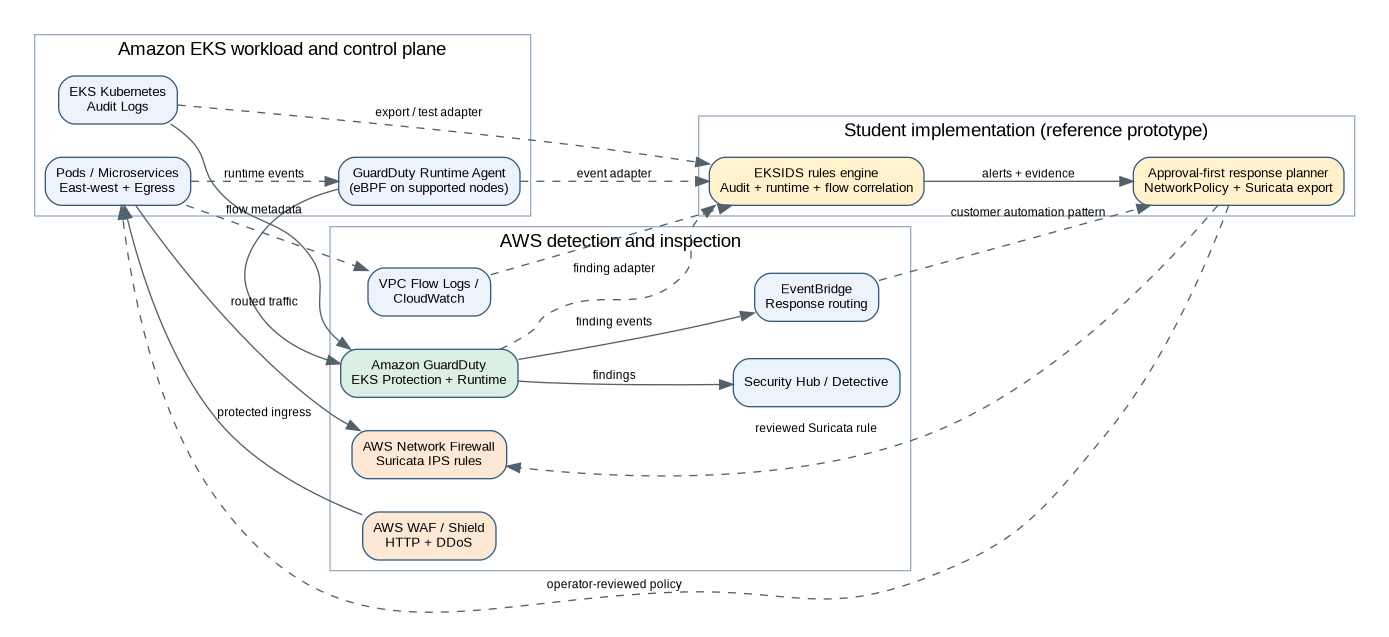
\includegraphics[width=0.96\textwidth]{../figures/architecture.png}
\caption{AWS EKS security architecture and the student-implemented event correlation/response component. The design is a synthesis, not a claim of a single AWS-published reference topology.}
\label{fig:arch}
\end{figure*}

\subsection{Event model and detection rules}
The engine accepts four event families: (i) Kubernetes audit events with actor, verb, resource and object context; (ii) runtime events resembling Falco/Tetragon records; (iii) network-flow records with source, destination, port and byte counts; and (iv) GuardDuty/EventBridge finding envelopes. Each record carries timestamp and, where available, namespace, Pod and actor identity.

Table~\ref{tab:rules} summarizes the implemented rules. Network scan detection maintains a sliding time window per Pod identity. A correlation rule escalates suspicious shell execution followed by known-bad egress from the same Pod within 60 seconds. Other rules evaluate security-sensitive Kubernetes API operations, runtime process/file events, known-bad egress indicators and large external transfers. Alerts contain a stable rule identifier, severity, evidence and a response suggestion. Rules are intentionally deterministic and inspectable.

\begin{table}[t]
\caption{Implemented detection rules}\label{tab:rules}
\centering\small
\begin{tabular}{p{0.17\columnwidth}p{0.73\columnwidth}}
\toprule
Rule & Detection condition \\
\midrule
K8S-001 & Privileged Pod or sensitive hostPath workload creation \\
K8S-002 & Kubernetes Secret get/list/watch activity \\
K8S-003 & Role binding granting cluster-admin \\
K8S-004 & Exec into kube-system or kube-public \\
RT-001/2 & Shell/network utility execution or sensitive-file access \\
NET-001 & At least eight distinct destination ports in a 60-s Pod window \\
NET-002 & Outbound connection to configured threat-intelligence IP \\
NET-003 & Large outbound flow to an external address \\
CORR-001 & Shell execution and known-bad egress from same Pod within 60 s \\
AWS-GD & Normalize and triage an upstream GuardDuty finding \\
\bottomrule
\end{tabular}
\end{table}

\subsection{Response planner and safety controls}
For selected Pod-level runtime/network alerts, the planner creates a scoped Kubernetes NetworkPolicy with ingress and egress isolation intent. It also exports a Suricata-compatible drop-rule string for a configured external indicator, suitable for review before insertion into an AWS Network Firewall stateful rule group. The implementation defaults to recommendation-only mode. It does not call AWS or Kubernetes APIs, and it does not automatically apply rules.

This boundary is important. NetworkPolicy is additive and depends on a supporting CNI; a generated deny policy is not a universal override of other allow policies. It cannot revoke IAM permissions, rotate credentials, or remediate a compromised node. Those response paths require separate IAM/RBAC, credential-management and host-level controls. Fig.~\ref{fig:response} shows the approval-first operational sequence.

\begin{figure}[t]
\centering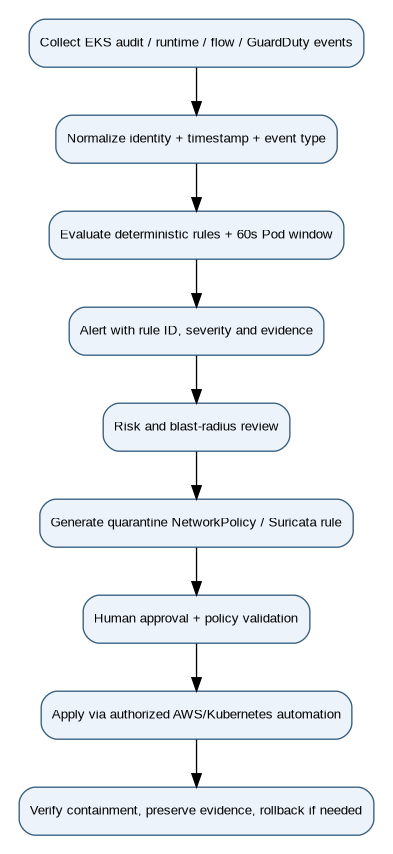
\includegraphics[width=0.95\columnwidth]{../figures/response.png}
\caption{Approval-first detection and response workflow.}
\label{fig:response}
\end{figure}

\section{Implementation}
The reference implementation is written in Python and organized as a small package. \texttt{engine.py} processes normalized events and emits structured alerts. A bounded deque stores recent network flows per Pod for scan detection. \texttt{policy.py} generates a quarantine NetworkPolicy only when the operator supplies verified workload labels, and exports a Suricata rule string. \texttt{replay.py} replays newline-delimited JSON fixtures. \texttt{evaluate.py} generates controlled cases and compares multi-source detection with audit-only, runtime-only and network-only variants. Unit tests cover privileged workload detection, Secret access, scan bursts, known-bad egress, benign events, policy scoping and Suricata export.

The system intentionally uses no trained model. This makes the decision path deterministic and supports direct explanation during incident review. The AWS mapping is an integration design: actual production deployment would connect CloudWatch/GuardDuty/EventBridge exports to the adapters and would use a separately authorized action executor.

\section{Experimental Evaluation}
\subsection{Method}
The experiment uses seed 20261111 and 500 event cases: 400 benign and 100 attacks. Five attack families are represented: privileged/hostPath workload creation, Secret enumeration, suspicious shell execution, port-scan bursts and known-bad egress. To avoid a trivial perfect-score demonstration, 5\% of benign cases contain legitimate but sensitive administrative activity, and 20\% of attack cases have incomplete or non-indicative telemetry. A case is classified positive if at least one alert is generated. We compare four variants: audit-only, runtime-only, network-only and multi-source fused rules.

\subsection{Results}
Table~\ref{tab:results} reports precision, recall, F1 and false-positive rate. The multi-source detector reaches 0.80 recall and F1, compared with 0.31/0.411 for audit-only, 0.15/0.261 for runtime-only, and 0.34/0.507 for network-only. Its 0.05 false-positive rate reflects the intentionally included authorized-but-sensitive administrative actions. The single-source variants miss attacks whose evidence resides in another telemetry plane. Fig.~\ref{fig:metrics} visualizes the comparison.

\begin{table}[t]
\caption{Controlled event-replay results}\label{tab:results}
\centering\small
\begin{tabular}{lrrrr}
\toprule
Variant & Prec. & Recall & F1 & FPR \\
\midrule
Audit-only & 0.608 & 0.310 & 0.411 & 0.050 \\
Runtime-only & 1.000 & 0.150 & 0.261 & 0.000 \\
Network-only & 1.000 & 0.340 & 0.507 & 0.000 \\
Multi-source & 0.800 & 0.800 & 0.800 & 0.050 \\
\bottomrule
\end{tabular}
\end{table}

\begin{figure}[t]
\centering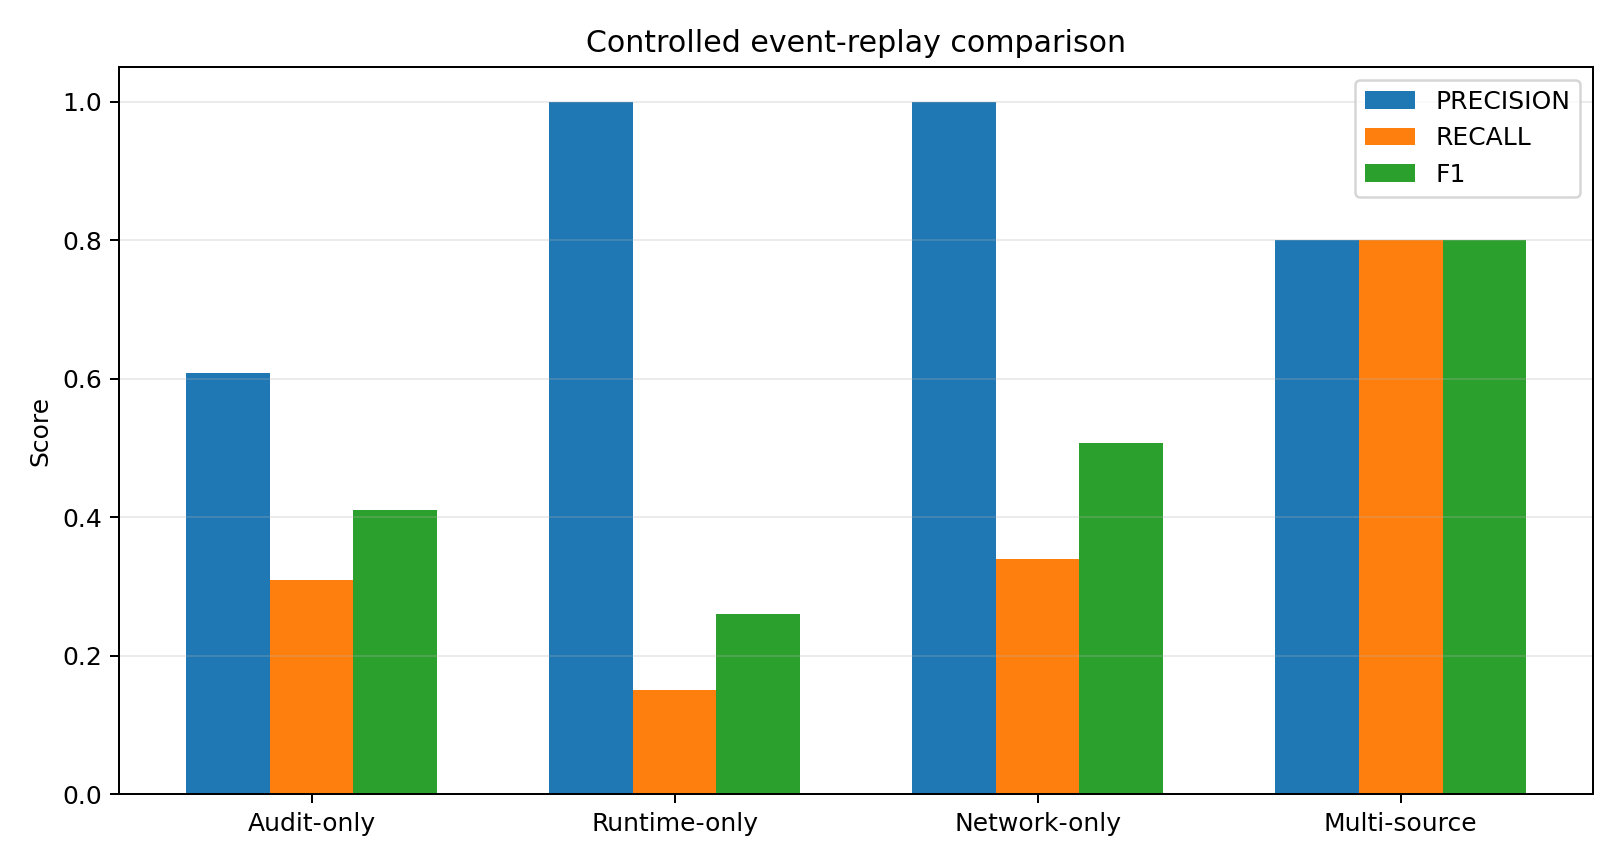
\includegraphics[width=0.98\columnwidth]{../figures/metrics.png}
\caption{Precision, recall and F1 for the controlled replay variants.}
\label{fig:metrics}
\end{figure}

The fused path's mean in-process processing time was approximately 0.0135 ms per case and p95 approximately 0.0435 ms on the execution machine. These figures exclude collection, delivery, cloud service processing, Kubernetes API calls, policy propagation, verification and rollback. They are not end-to-end latency or an SLO. Seven unit tests pass in the delivered project.

\section{Discussion and Limitations}
The experiment supports the engineering hypothesis that combining control-plane, runtime and network evidence improves coverage over a single telemetry source. It also shows a practical trade-off: sensitive operations can be legitimate, so a rule match should create an evidence-rich alert and review tier rather than an unconditional destructive action. The response planner therefore requires operator approval.

The main limitation is synthetic data. No live EKS cluster, GuardDuty sensor, AWS Network Firewall, eBPF agent, real malicious traffic or AWS cost measurement was used in the reported experiment. The chosen attack prevalence is artificial, and the event generator is designed to exercise known rules. The results cannot be generalized to production precision or recall. The runtime benchmark is local processing only. Future work should deploy a disposable EKS cluster, enable GuardDuty protections, collect real labelled events, measure event-to-alert and isolation latency, quantify node/agent overhead, test NetworkPolicy enforcement and rollback, and validate false positives on normal operational activity.

\section{Conclusion}
AWS EKS security is a layered system rather than a single IDS/IPS product. GuardDuty detects suspicious Kubernetes API and runtime behavior; Network Firewall provides stateful network IPS when traffic is routed through it; WAF/Shield protect application and DDoS surfaces; and Kubernetes NetworkPolicy limits Pod communication. EKS-IDS demonstrates a small, explainable customer-side bridge across these layers: it normalizes multi-source events, applies deterministic rules, correlates scan behavior over time, and generates approval-first response artefacts. Controlled replay indicates that multi-source rules improve coverage relative to isolated telemetry variants, while the synthetic nature of the experiment is stated explicitly. The work is intended as a reproducible teaching prototype and a foundation for live EKS evaluation.

\begin{thebibliography}{99}
\bibitem{nist190} M. Souppaya, J. Morello, and K. Scarfone, ``Application Container Security Guide,'' NIST SP 800-190, 2017, doi: 10.6028/NIST.SP.800-190.
\bibitem{nist207a} R. Chandramouli and Z. Butcher, ``A Zero Trust Architecture Model for Access Control in Cloud-Native Applications in Multi-Location Environments,'' NIST SP 800-207A, 2023, doi: 10.6028/NIST.SP.800-207A.
\bibitem{nist233} R. Chandramouli, Z. Butcher, and J. Callaghan, ``Service Mesh Proxy Models for Cloud-Native Applications,'' NIST SP 800-233, 2024, doi: 10.6028/NIST.SP.800-233.
\bibitem{her2025} H. Her et al., ``An In-Depth Analysis of eBPF-Based System Security Tools in Cloud-Native Environments,'' IEEE Access, 2025, doi: 10.1109/ACCESS.2025.3605432.
\bibitem{ryu2026} J. Ryu et al., ``Hybrid Runtime Detection of Malicious Containers Using eBPF,'' Computers, Materials \& Continua, 2026, doi: 10.32604/cmc.2025.074871.
\bibitem{oppong2026} A. Oppong-Asante et al., ``Runtime Detection of Attacks and Misconfigurations in Cloud-Native Kubernetes Environments Using eBPF Network Telemetry,'' Journal of Computer Virology and Hacking Techniques, 2026, doi: 10.1007/s11416-026-00671-8.
\bibitem{gdEKS} Amazon Web Services, ``GuardDuty EKS Protection,'' Amazon GuardDuty User Guide, accessed Nov. 2026. [Online]. Available: \url{https://docs.aws.amazon.com/guardduty/latest/ug/kubernetes-protection.html}
\bibitem{gdRuntime} Amazon Web Services, ``GuardDuty Runtime Monitoring,'' Amazon GuardDuty User Guide, accessed Nov. 2026. [Online]. Available: \url{https://docs.aws.amazon.com/guardduty/latest/ug/runtime-monitoring.html}
\bibitem{gdEKSRuntime} Amazon Web Services, ``How Runtime Monitoring works with Amazon EKS clusters,'' accessed Nov. 2026. [Online]. Available: \url{https://docs.aws.amazon.com/guardduty/latest/ug/how-runtime-monitoring-works-eks.html}
\bibitem{nfwRules} Amazon Web Services, ``Managing your own rule groups in AWS Network Firewall,'' accessed Nov. 2026. [Online]. Available: \url{https://docs.aws.amazon.com/network-firewall/latest/developerguide/rule-groups.html}
\bibitem{nfwStateful} Amazon Web Services, ``Working with stateful rule groups in AWS Network Firewall,'' accessed Nov. 2026. [Online]. Available: \url{https://docs.aws.amazon.com/network-firewall/latest/developerguide/stateful-rule-groups-ips.html}
\bibitem{eksNetwork} Amazon Web Services, ``Network security,'' Amazon EKS Best Practices Guide, accessed Nov. 2026. [Online]. Available: \url{https://docs.aws.amazon.com/eks/latest/best-practices/network-security.html}
\bibitem{sccThreat} Google Cloud, ``Threat detection in Security Command Center,'' accessed Nov. 2026. [Online]. Available: \url{https://docs.cloud.google.com/security-command-center/docs/overview-threats}
\bibitem{gkeThreat} Google Cloud, ``GKE threat findings,'' Security Command Center documentation, accessed Nov. 2026. [Online]. Available: \url{https://docs.cloud.google.com/security-command-center/docs/gke-threats}
\bibitem{gkeNetwork} Google Cloud, ``Understand network security in GKE,'' accessed Nov. 2026. [Online]. Available: \url{https://docs.cloud.google.com/kubernetes-engine/docs/concepts/about-security-in-networking}
\end{thebibliography}
\end{document}
